Our goal in this work is to optimize the performance of tool calling in LM-based agents by speculating tool calls and executing them before they are needed. We propose two approaches for speculative tool calling: strictly client-side speculation that reduces tool latency and an inference-engine-side speculative algorithm that reduces both decode and prefill time.

In traditional tool calling, the user first submits a prompt to an API endpoint inference server.
The server starts processing the prompt and then returns the generated tokens to the user when it hits a stop token.
This could be the end of the sequence or a tool call token.
When the user receives the response from the server, they check why the generation stopped (e.g. tool call, end of sequence, timeout, max tokens, API credits) and, if it is a tool call, then they run the tool locally using the tool parameters generated by the model.
Once the tool completes the user passes the output back to the API and the LM can keep generating using the tool output.
This process is detailed in \Cref{alg:baseline-tool}.

\begin{algorithm}[h]
\caption{Baseline Tool-Calling (Client-side, No Speculation)}
\label{alg:baseline-tool}
\begin{algorithmic}[1]
    \Require Prompt $p$, chat history $H$, tools $\mathcal{T}$, main LM $\mathcal{M}$
    \Ensure Final model output $y$
    \State $r \gets \textsc{CallAPI}(\mathcal{M}, p, H, \mathcal{T})$
    \If{$\textsc{HasToolCall}(r)$}
      \State $\tau \gets \textsc{ExtractToolCall}(r)$
      \State $v \gets \textsc{RunTool}(\tau)$
      \State $H' \gets H \cup \{(\tau, v)\}$ \Comment{append tool result to history}
      \State $y \gets \textsc{CallAPI}(\mathcal{M}, p, H', \mathcal{T})$ \Comment{return final answer}
    \Else
      \State $y \gets \textsc{Render}(r)$ \Comment{no tool call; use first pass}
    \EndIf
    \State \Return $y$
\end{algorithmic}
\end{algorithm}

\subsection{Client-side Speculative Tool Calling}\label{sec:spec-tool:user}

\begin{figure*}[t]
    \centering
    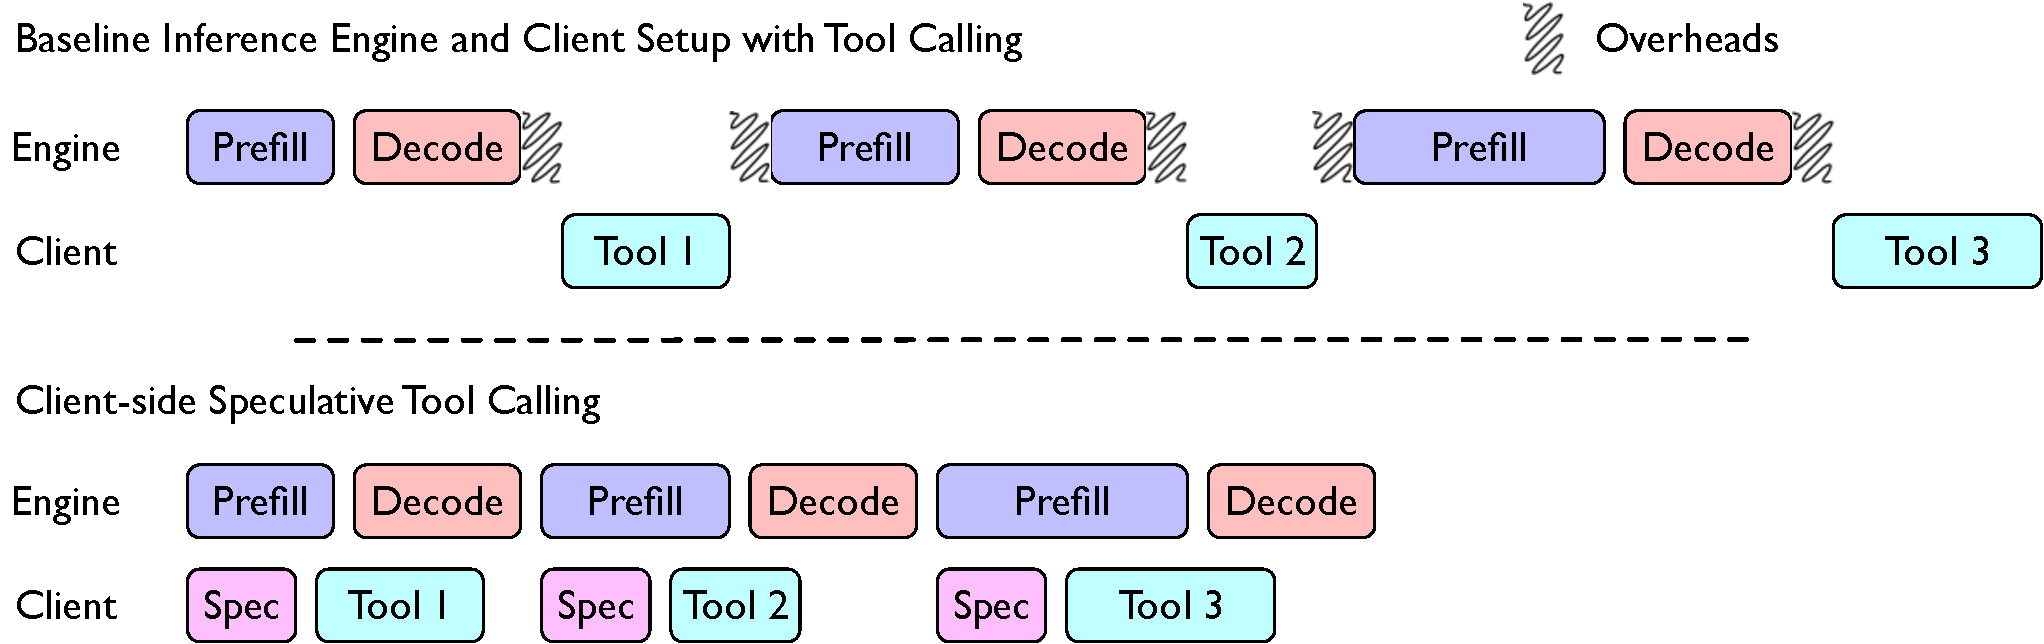
\includegraphics[width=0.8\textwidth]{figs/client-side}
    \caption{Overview of the client-side approach for speculative tool calling. Our approach speculates tool calls and overlaps their execution with generation.}
    \label{fig:client-side}
\end{figure*}

We expand on the traditional tool calling approach with speculative tool calling on the client side as described in \Cref{alg:spec-tool-cache}.
In this approach we asynchronously send our prompt to two API endpoints: the main model $\mathcal{M}$ and a speculative model $\mathcal{S}$.
The speculative model is much smaller and should return estimated tool calls with much lower latency than the main model.
When $\mathcal{S}$ returns a tool call, we asynchronously launch the tool and start executing it.
We store a {\it future} for its result in a tool cache.
When $\mathcal{M}$ finally returns generated tokens, we check if a tool call is required.
If it is required and there is a future for that tool call in the cache, we wait on the future instead of relaunching the tool. Figure~\ref{fig:client-side} provides an overview of our approach.
We can further increase speculation by launching several speculative model instances (represented by $\lambda$ in \Cref{alg:spec-tool-cache}).

\begin{algorithm}[!htbp]
\caption{Client-side Speculative Tool-Calling}
\label{alg:spec-tool-cache}
\begin{algorithmic}[1]
    \Require Prompt $p$, chat history $H$, tools $\mathcal{T}$, sampling factor $\lambda$, main LLM $\mathcal{M}$, speculative LM $\mathcal{S}$
    \Ensure Final model output $y$
    \State $C \gets \textsc{EmptyMap}()$ \Comment{cache: \textit{tool call} $\mapsto$ \textit{future}}
    \State \textbf{spawn} $h_m \gets \textsc{CallAPI}(\mathcal{M}, p, H, \mathcal{T})$ \Comment{start main generation asynchronously}
    \For{$i \gets 1$ to $\lambda$} \Comment{speculative samples in parallel}
      \State \textbf{spawn}:
      \Statex \hspace{1.2em} $s_i \gets \textsc{CallAPI}(\mathcal{S}, p, H, \mathcal{T})$
      \If{$\textsc{HasToolCall}(s_i)$}
        \State $\tau \gets \textsc{ExtractToolCall}(s_i)$
        \If{$\tau \notin C$}
          \State $C[\tau] \gets \textsc{StartToolAsync}(\tau)$ \Comment{begin executing tool; returns a future}
        \EndIf
      \EndIf
    \EndFor
    \\
    \State $r_m \gets \textbf{await}\; h_m$ \Comment{wait for main generation}
    \\
    \If{$\textsc{HasToolCall}(r_m)$}
      \State $\tau_m \gets \textsc{ExtractToolCall}(r_m)$
      \If{$\tau_m \in C$}
        \State $v \gets \textbf{await}\; C[\tau_m]$ \Comment{reuse if available}
      \Else
        \State $v \gets \textsc{RunTool}(\tau_m)$ \Comment{execute tool now}
      \EndIf
      \State $H' \gets H \cup \{(\tau_m, v)\}$ \Comment{append tool result to history}
      \State $y \gets \textsc{CallAPI}(\mathcal{M}, p, H', \mathcal{T})$ \Comment{call $\mathcal{M}$ with result}
    \Else
      \State $y \gets \textsc{Render}(r_m)$ \Comment{no tool call}
    \EndIf
    \\
    \State \Return $y$
\end{algorithmic}
\end{algorithm}

It is important to note that we can only speculate \emph{stateless, cheap} tools.
If a tool or function requires or modifies state, then speculating it is impossible without some undo or rollback mechanism.
This is an interesting potential optimization but out of the scope of this paper.
Further, if a tool call is expensive, either in dollar costs or execution time, it is undesirable to launch many attempts of the tool ahead of time if they will not be correct.
Fortunately, many common agent tools, such as web-search and file access, are both cheap and stateless providing ample opportunity for speculation.

\subsubsection{Analysis of Client-side Speculation}\label{sec:client-side-analysis}

We examine a particular case where the user is repeatedly calling the API and receiving a tool call from the API each time.
This closely mimics the usage pattern of most AI agents and is, thus, a reasonable case to consider.
The times to process $N$ requests from the user in the standard (\Cref{alg:baseline-tool}) and speculative (\Cref{alg:spec-tool-cache}) case are shown below.

\vspace{1.5em}
\begin{align}
    T_{\mathtt{standard}} &= N (\eqnmarkbox[MidnightBlue]{G1}{G} + \eqnmarkbox[WildStrawberry]{T1}{T}) \nonumber \\
    T_{\mathtt{spec}} &= \eqnmarkbox[Orchid]{a1}{\alpha} N \max\{\eqnmarkbox[MidnightBlue]{G2}{G},\eqnmarkbox[OliveGreen]{g}{g}+\eqnmarkbox[WildStrawberry]{T2}{T}\} + (1-\eqnmarkbox[Orchid]{a2}{\alpha})N(\eqnmarkbox[MidnightBlue]{G3}{G}+\eqnmarkbox[WildStrawberry]{T3}{T})
\end{align}
\annotate[yshift=1em]{above,left}{G1}{avg. $\mathcal{M}$\\ generation time}
\annotate[yshift=1em]{above,right}{T1}{avg. tool call time}
\annotate[yshift=0.5em,xshift=0.3em]{above,right}{g}{avg. $\mathcal{S}$ generation time}
\annotatetwo[yshift=-0.8em]{below}{a1}{a2}{$\mathcal{S}$ acceptance rate}
\vspace{1em}

The left term in $T_{\mathtt{spec}}$ is the case where the speculative model was correct and, thus, we only wait $g+T$ for the tool to complete.
The maximum is necessary since we still need to wait on $\mathcal{M}$ to complete to validate the right tool call, so if $g+T<G$, then we still have to wait $G$.
Assuming $T$, $g$, $G$, and $N$ are positive, non-zero and $0\le\alpha\le1$ we can further analyze the speedup of the speculative algorithm.
\begin{align}
    S_{\mathtt{spec}} =& \frac{T_{\mathtt{standard}}}{T_{\mathtt{spec}}} &> 1 \nonumber \\
  =& \frac{G + T}{\alpha \max\{G, g+T\} + (1-\alpha)(G+T)} &> 1 \label{eq:client-alg-speedup}
\end{align}
\begin{align}
  \text{If $g+T \ge G$, then} \nonumber \\
  S_{\mathtt{spec}} =& \frac{G+T}{\alpha(g-G)+G+T} &> 1 \nonumber \\
  & \alpha(g-G)+G+T &< G+T  \nonumber \\
  & \alpha(g-G) &<0\nonumber \\
    \implies & \alpha > 0 \textrm{ and } g < G \label{eq:client-alg-condition}
\end{align}


We can immediately see that $S_{\mathtt{spec}}>1$ when $\mathcal{S}$ has a non-zero acceptance rate and $\mathcal{S}$ is faster than $\mathcal{M}$. 
The case where $g+T<G$ is ignored, since this trivially leads to speedups greater than 1 when $\alpha>0$ (i.e. speculation and tool calling are completely masked by the main models generation time, so any correct speculation should lead to speedups).
Based on \Cref{eq:client-alg-condition} \emph{to achieve speedups with speculative tool calling on the client side we need to find a speculation model $\mathcal{S}$ that is faster than the main model $\mathcal{M}$ and has a tool speculation accuracy greater than 0}.

Another key insight from \Cref{eq:client-alg-speedup} is that $S_{\mathtt{spec}} < 2$, i.e. \emph{the maximum speedup we can achieve in this approach is 2.
Furthermore, the speedup approaches 2 as $g\rightarrow 0$}.
\Cref{fig:client-alg-model-speedups} shows the distribution of $S_{\textrm{spec}}$ across values of $\alpha$, $g/G$, and $T$.
We see the above trends, i.e. that $S_{\textrm{spec}}\rightarrow 2$ as $g\rightarrow 0^+$ and $S_{\textrm{spec}}<2$, but also that we only see large speedups for values of $T$ near $G$.
As $T\rightarrow 0$ the total time is predominantly dominated by $G$ and as $T\rightarrow \infty$ it is dominated by the tool call.
Thus, when $T\approx G$ there are more values of $\alpha$ and $g/G$ where we can see substantial benefits.
The above insights are also proven below in \Cref{lemma:client-alg-proof}.

\begin{figure*}[t]
    \centering
    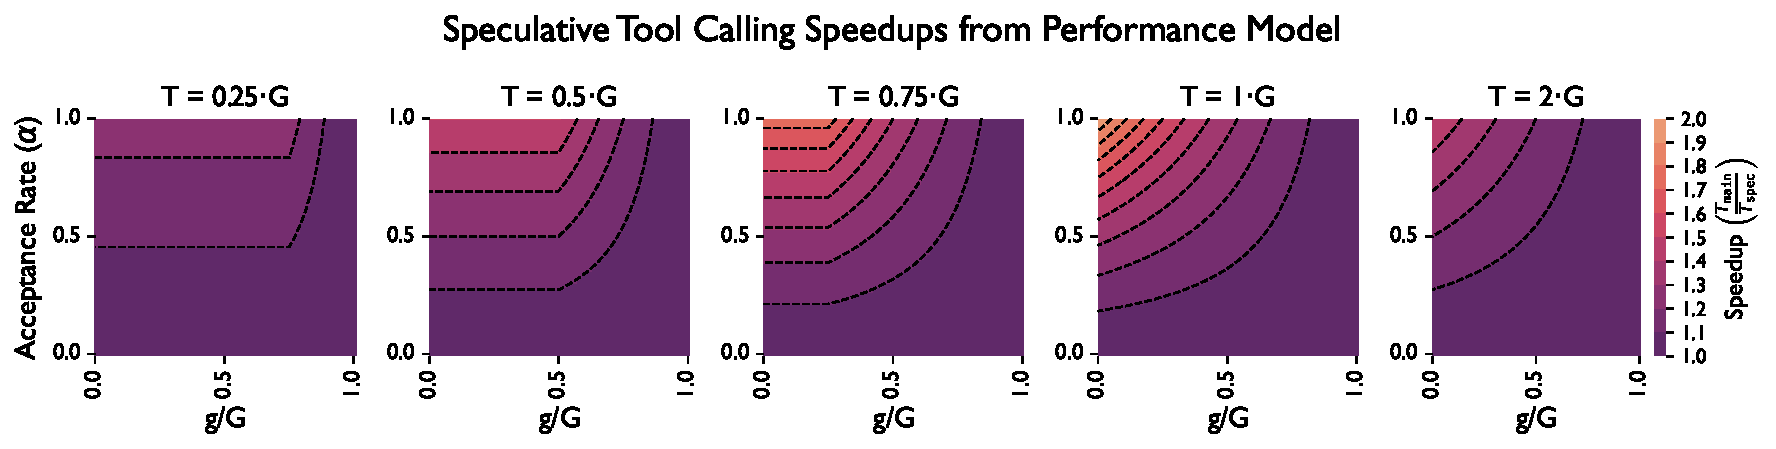
\includegraphics[width=0.9\textwidth]{figs/client-side-spec-model-speedup-heatmap}
    \caption{Distribution of speculative tool calling speedups for the client-side algorithm across various acceptance rates, generation times, and tool call times. $\alpha$ is the acceptance rate of the speculative model $\mathcal{S}$, $g/G$ is the ratio of generation time between the speculative and main models, and $T$ is the tool call time. Values of $T\approx G$, $\alpha > 0.5$, and $g/G < 0.5$ yield higher speedups, but are ultimately limited at a 2$\times$ speedup. \label{fig:client-alg-model-speedups}}
\end{figure*}

\begin{lemma}[Speedup bound] \label{lemma:client-alg-proof}
Let $G,g,T>0$, $g<G$, and $\alpha\in[0,1]$. Define
\[
S_{\mathrm{spec}}(\alpha)
=\frac{G+T}{\alpha\,\max\{G,\,g+T\}+(1-\alpha)(G+T)}.
\]
Then:
\begin{enumerate}
  \item $S_{\mathrm{spec}}(\alpha)$ is strictly increasing in $\alpha$, hence $S_{\mathrm{spec}}(\alpha)>1$ for all $\alpha>0$.
  \item The maximum over $\alpha\in[0,1]$ is attained at $\alpha=1$ and equals
  \[
  S_{\max}=\frac{G+T}{\max\{G,\,g+T\}}.
  \]
  \item Moreover,
  \[
  S_{\max}\le \frac{2(G+T)}{G+g+T}
  = 2-\frac{2g}{G+g+T} \;<\; 2.
  \]
  In particular, the supremum $2$ is approached only in the limit $g\to 0^+$.
\end{enumerate}
\end{lemma}

\begin{proof}
Let $M:=\max\{G,\,g+T\}$ and write
\begin{align}
S_{\mathrm{spec}}(\alpha) =& \frac{G+T}{\alpha M+(1-\alpha)(G+T)} \nonumber \\
=& \frac{G+T}{(G+T)+\alpha\,(M-(G+T))}. \nonumber 
\end{align}
Set $\Delta:=M-(G+T)$. Since $M\le G+T$, we have $\Delta\le 0$, with strict inequality because $G,g,T>0$.

\smallskip
\noindent\textbf{(1)} Since $M\le G+T$ and $G,g,T,\alpha>0$, the denominator of $S_{\mathrm{spec}}(\alpha)$ is strictly decreasing as $\alpha$ increases.
Thus, we can conclude that $S_{\mathrm{spec}}(\alpha)$ is strictly increasing with $\alpha$. Furthermore, since $S_{\mathrm{spec}}(0)=1$ it follows that $S_{\mathrm{spec}}(\alpha)>1$ for all $\alpha>0$. 


\smallskip
\noindent\textbf{(2)} Monotonicity implies the maximum over $[0,1]$ occurs at $\alpha=1$, giving
\[
S_{\max}=S_{\mathrm{spec}}(1)=\frac{G+T}{M}=\frac{G+T}{\max\{G,\,g+T\}}.
\]

\smallskip
\noindent\textbf{(3)} For any $a,b>0$, $\max\{a,b\}\ge \tfrac{a+b}{2}$. 
Applying this with $a=G$ and $b=g+T$,
\begin{align}
S_{\max} =& \frac{G+T}{\max\{G,\,g+T\}} \nonumber \\
\le& \ \frac{G+T}{\tfrac{G+(g+T)}{2}}
= \frac{2(G+T)}{G+g+T}
= 2-\frac{2g}{G+g+T} \nonumber \\
<& \  2, \nonumber
\end{align}
where the strict inequality uses $g>0$. This proves the stated bound and its strictness.
\end{proof}

\begin{observationbox}{Client-side speculation limit}
Client-side speculative tool calling is limited at a $2\times$ speedup: we can only
hide one of the two dominant phases (generation or tool execution). 
For a good speculative model (fast and accurate), the best gains occur when the tool latency $T$ is approximately equal to the main model generation time $G$.
\end{observationbox}



\subsection{Engine-side Speculative Tool Calling}\label{sec:spec-tool:prefill}


\begin{figure*}[t]
    \centering
    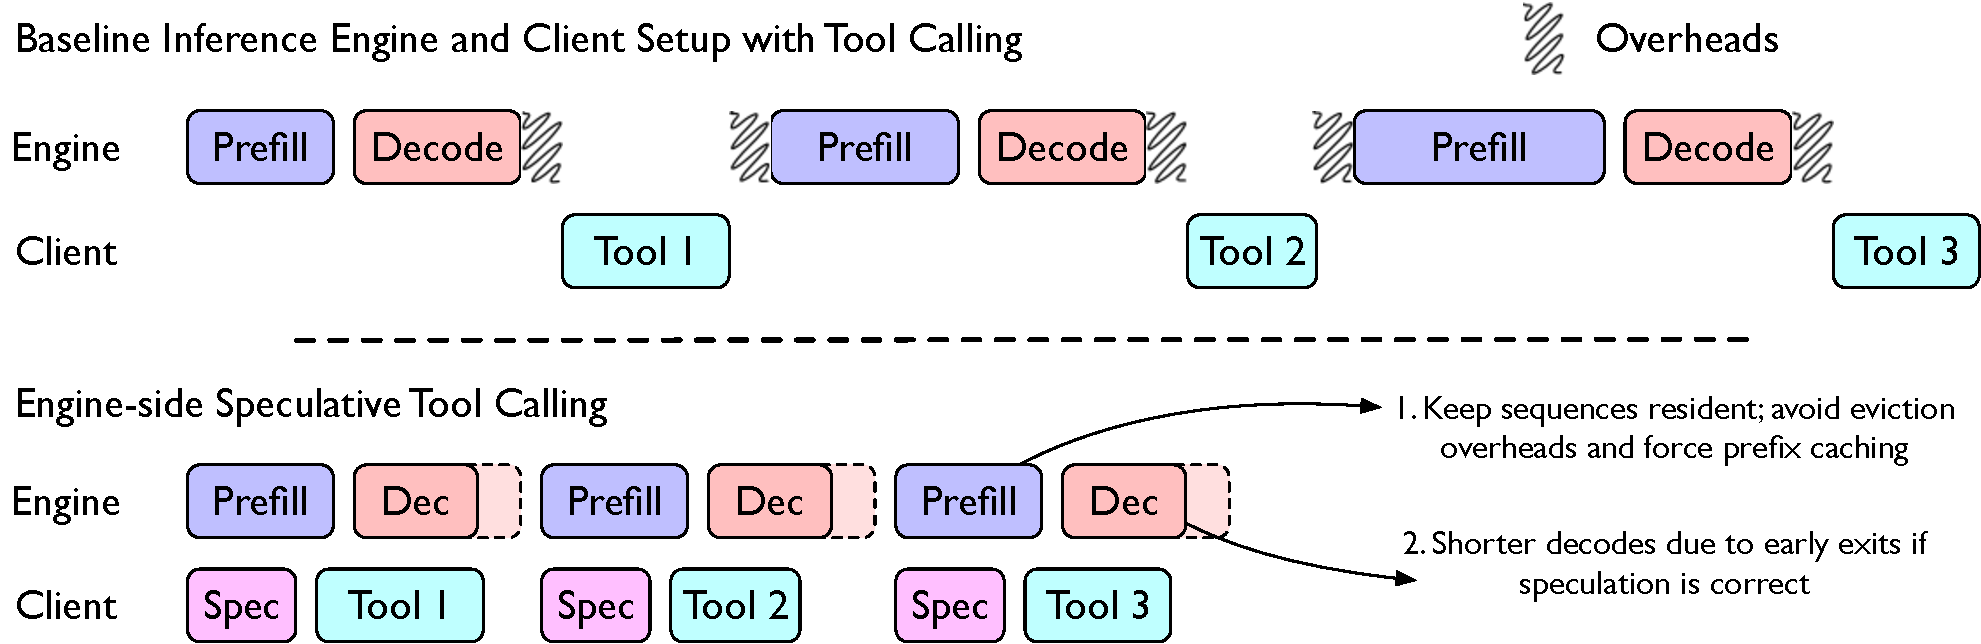
\includegraphics[width=0.8\textwidth]{figs/engine-side}
\caption{Overview of our proposed engine-side algorithm for speculative tool calling for agents. First, our approach speculates tool calls and overlaps their execution with generation. Second, if speculated tool calls are available before the target model finishes decoding it, then we can validate the tool call in a single forward pass and early exit decoding. Finally, by posting speculated tool outputs to the server, we prevent the prefill time from continuing to grow and remove overheads from removing the prompt from the batch.}
    \label{fig:engine-side}
\end{figure*}

Next, we present our approach of moving our speculative tool calling method from the client to the engine. First, we present how a non-speculative inference engine with tool calling works in 
Algorithm \ref{alg:engine-baseline}. The engine repeatedly ingests new requests from the input queue into an active batch. For each sequence in the batch, it first encodes the prompt to produce the first token (prefill) and then generates subsequent tokens (decode). When a stop token (end of sequence or tool call token) is produced, the engine stops generation. If the stop token is a tool call token, the engine returns the tool call to the client, and evicts the sequence from the active batch. Its KV-cache is discarded unless prefix-caching is enabled.



\begin{algorithm}[!htbp]
\caption{Baseline Inference Engine: Batch Decode with Evict-then-Refill on Tool Calls}
\label{alg:engine-baseline}
\begin{algorithmic}[1]
\Require Input queue $\mathsf{Q}$, model $\mathcal{M}$, batch size $K$
\State $\mathsf{B} \gets \emptyset$ \Comment{active batch of sequences}
\While{\textsc{ServiceRunning}()}
  \State \textbf{fill} $\mathsf{B}$ from $\mathsf{Q}$ up to $K$ ready requests
  \ForAll{$s \in \mathsf{B}$}
  \If {$s.\textsc{status} = \textsc{New}$}
    \State $t \gets \textsc{Prefill}(\mathcal{M}, s)$ \Comment{first token}
    \State $s.\textsc{status} \gets \textsc{Decode}$
    \ElsIf {$s.\textsc{status} = \textsc{Decode}$}
  \State $t \gets \textsc{DecodeStep}(\mathcal{M}, s)$ \Comment{get next token}
    \EndIf
    \State
      \If{$\textsc{IsStop}(t)$}
        \State \textsc{EmitToClient}$(s, \text{final})$
        \State \textsc{Evict}$(\mathsf{B}, s)$ \Comment{KV-cache maybe dropped}
      \EndIf
    \EndFor
  \State \textbf{ingest} any new/follow-up requests from client (e.g. tool results) into $\mathsf{Q}$
\EndWhile
\end{algorithmic}
\end{algorithm}


The engine-side speculative approach adds a tool cache maintained by the inference engine. Similar to the previous approach, the client spawns multiple speculative model instances and launches tools asynchronously. However, instead of storing futures, it waits for each tool execution to finish and then submits the result to the engine, indexed by a normalized key (tool name + canonicalized arguments) and the request ID. On the engine side, we introduce two optimizations based on the tool cache. When a tool start token (the first token indicating that the model is about to produce a tool invocation) is detected for a sequence, the engine performs a cache lookup using the request ID and tool name.  
If found, the argument tokens of the latest matching tool call are injected as draft tokens and validated through standard speculative sampling. This ensures correctness and potentially avoids the need to generate the tool call arguments (early exit decoding). When a tool end token (the token indicating that the full tool call has been emitted) is detected, the engine looks up the full key. On a cache hit, the tool result is appended and the KV-cache updated so decoding can continue without eviction. Otherwise, the engine falls back to baseline behavior and emits the tool call to the client.~\Cref{fig:engine-side} provides an overview of this approach. The client and engine behaviors under this approach are described in Algorithms~\ref{alg:client-speculative} and~\ref{alg:engine-speculative}, respectively.

\begin{algorithm}[h]
\caption{Client with Speculative Tool Execution and Cache Submission}
\label{alg:client-speculative}
\begin{algorithmic}[1]

\Require Prompt $p$, chat history $H$, tools $\mathcal{T}$, main LM API endpoint $\mathsf{E}$, speculative LLM $\mathcal{S}$, samples $\lambda$
\Ensure Final output $y$
\State $(h, \mathit{rid}) \gets \textsc{CallAPI}(\mathsf{E}, p, H, \mathcal{T})$ \Comment{start main request; get request id}
\For{$i \gets 1$ to $\lambda$} \Comment{launch speculative samples}
  \State \textbf{spawn} $s_i \gets \textsc{CallLLM}(\mathcal{S}, p, H, \mathcal{T})$
  \If{$\textsc{HasToolCall}(s_i)$}
    \State $\tau \gets \textsc{ExtractToolCall}(s_i)$
    \State $f \gets \textsc{StartToolAsync}(\tau)$
    \State \textbf{spawn} \textsc{OnReady}$(f)$:
    \Statex \hspace{4em} $v \gets \textbf{await}\; f$
    \Statex \hspace{4em} $k \gets \textsc{CanonKey}(\tau)$ \Comment{normalize: tool name + canonicalized args}
    \Statex \hspace{4em} \textsc{SubmitToolCache}$(\mathsf{E}, \mathit{rid}, k, v)$
  \EndIf
\EndFor
\State
\State $r \gets \textbf{await}\; h$ \Comment{receive result (may be final or a tool call)}
\State
\If{$\textsc{HasToolCall}(r)$}
  \Comment{cache miss path: engine did \emph{not} find value in its cache}
  \State $\tau^\star \gets \textsc{ExtractToolCall}(r)$
  \State $v^\star \gets \textsc{RunTool}(\tau^\star)$
  \State $H' \gets H \cup \{(\tau^\star, v^\star)\}$
  \State $r \gets \textsc{CallAPI}(\mathsf{E}, p, H', \mathcal{T})$ \Comment{continue normal loop}
  \While{$\textsc{HasToolCall}(r)$}
    \State $\tau \gets \textsc{ExtractToolCall}(r)$
    \State $v \gets \textsc{RunTool}(\tau)$; $H' \gets H' \cup \{(\tau, v)\}$
    \State  $r \gets \textsc{CallAPI}(\mathsf{E}, p, H', \mathcal{T})$
  \EndWhile
\EndIf
\State $y \gets \textsc{Render}(r)$
\State \Return $y$
\end{algorithmic}
\end{algorithm}

\begin{algorithm}[h!]
\caption{Inference Engine with Tool Cache} %
\label{alg:engine-speculative}
\begin{algorithmic}[1]
\Require Input queue $\mathsf{Q}$, model $\mathcal{M}$, batch size $K$, tool cache $\mathsf{C}$ keyed by (request id, canon key) and (request id, tool name)
\State $\mathsf{B} \gets \emptyset$
\While{\textsc{ServiceRunning}()}
  \State \textsc{AsyncUpdate}($\mathsf{C}$) \Comment{from \textsc{SubmitToolCache}}
  \State \textbf{fill} $\mathsf{B}$ from $\mathsf{Q}$ up to $K$
  \ForAll{$s \in \mathsf{B}$}
  \If {$s.\textsc{status} = \textsc{New}$}
    \State $t \gets \textsc{Prefill}(\mathcal{M}, s)$; $s.\textsc{status} \gets \textsc{Decode}$
    \ElsIf{$s.\textsc{status} = \textsc{Decode}$}
      \State $t \gets \textsc{DecodeStep}(M, s)$
    \EndIf
    \State
     \If{$\textsc{IsToolCallStart}(t)$}
        \State $\eta \gets \textsc{ExtractToolName} (s, t)$
        \If{$\mathsf{C}.\textsc{Has}(\textit{rid}(s),\eta)$}
        \State $c \gets \mathsf{C}.\textsc{GetToolCall}(\textit{rid}(s),\eta)$
        \State $t \gets \textsc{SpeculativeSample}(\mathcal{M}, s, c)$ \Comment{Validate tool call tokens and update KV cache}
        \EndIf
        \ElsIf{$\textsc{IsToolCallEnd}(t)$}
        \State $\tau \gets \textsc{ExtractToolCall}(s, t)$
        \State $k \gets \textsc{CanonKey}(\tau)$
        \If{$\mathsf{C}.\textsc{Has}(\textit{rid}(s), k)$} \Comment{cache hit}
          \State $v \gets \mathsf{C}.\textsc{GetToolResult}(\textit{rid}(s), k)$
          \State $t \gets \textsc{PrefillToolResult}(\mathcal{M}, s, \tau, v)$ \Comment{append tool result tokens to KV cache}
        \EndIf
        \EndIf
      \State
      \If{$\textsc{IsStop}(t)$} \Comment{cache miss/other stop token}
        \State \textsc{EmitToClient}$(s, \text{final})$ 
        \State \textsc{EvictFromBatch}$(\mathsf{B}, s)$
      \EndIf
    \EndFor
  \State \textbf{ingest} \textsc{New} client requests into $\mathsf{Q}$
\EndWhile
\end{algorithmic}
\end{algorithm}






\subsubsection{Analysis of Engine-side Speculation}\label{sec:engine-side-analysis}

In the traditional case of tool calling, where the user receives the tool parameters, runs it, and calls the API again, we can model the runtime from the inference engine's perspective as shown in \Cref{eq:spec-engine-vanilla} for $K$ consecutive agent turns.
This accounts for the prefill and decode phase of each turn where $X_i$ tokens are prefilled, $R_i$ reasoning tokens are decoded, and $t_i$ tool call tokens are decoded.
Then the tool is called for $T_i$ seconds after which the tool call and output ($t_i+t_{o,i}$ tokens) are sent back to the API.
Finally, the entire history and new tool calls will be prefilled again, so we sum them in the $X_i$ recursive term.
In between these phases there is also overhead, $o$, to passing the prompts through the API via HTTP and loading it into the running batch.

\vspace{1em}
\begin{equation}\label{eq:spec-engine-vanilla}
    T_{\textrm{vanilla}} = 
    2K\eqnmarkbox[MidnightBlue]{o1}{o} + 
    \eqnmarkbox[Apricot]{p1}{\varphi} \sum_{i=1}^K X_i + 
    \eqnmarkbox[OliveGreen]{d1}{\delta} \sum_{i=1}^K 
        \left(
            \eqnmarkbox[Orchid]{r1}{R_i} + 
            \eqnmarkbox[Mahogany]{t1}{t_i}
        \right) + 
    \sum_{i=1}^K \eqnmarkbox[Red]{T1}{T_i}
\end{equation}
\annotate[yshift=1.2em,xshift=0em]{above,left}{o1}{API and eviction\\overheads}
\annotate[yshift=-1.2em]{below,left}{p1}{Prefill rate (s/tok)}
\annotate[yshift=1.2em]{above, left}{d1}{Decode rate (s/tok)}
\annotate[yshift=1.2em]{above, left}{T1}{Tool duration (s)}
\annotate[yshift=-1.2em]{below, left}{r1}{Reasoning tokens}
\annotate[yshift=-1.2em]{below, right}{t1}{Tool call tokens}
\vspace{1em}


such that

\begin{equation}
    X_{i+1} = X_i + t_i + t_{o,i}, \quad X_1 = \textrm{initial prompt tokens} \nonumber
\end{equation}

Here we assume that (1) reasoning tokens from previous turns are not included in the prefill for future turns as is typical for most commercial APIs and (2) 
there are no additional outputs alongside the tool call during each turn. The former assumption is generally true across API models, while the latter depends on 
how the agent framework is implemented (directly using tools versus thought-actions as in SWE-Agent). Despite this, our model is without loss of generality,
since you can absorb these extra decode tokens into the $t_i$ term.

Note that in the case of prefix-caching we can express the time as shown in \Cref{eq:spec-engine-pref-cache}. Here we do not have to repeat prefills for
tokens we have already populated into the KV-cache.

\begin{equation}\label{eq:spec-engine-pref-cache}
    T_{\textrm{cached}} = 2Ko + \varphi\left(X_1 + \sum_{i=1}^{K}(t_i+t_{o,i})\right) + \delta\sum_{i=1}^{K}(R_i+t_i) + \sum_{i=1}^{K} T_i
\end{equation}










Next we consider the three primary optimizations: (1) speculating tools prior to execution (\emph{O1}), (2) validating cached tool calls with a single forward pass during decoding (\emph{O2}), and (3) avoiding eviction and duplicate prefilling for tool calls where the output is already available (\emph{O3}).
The first optimization (\emph{O1}) can save us up to $\sum_{i=1}^K T_i$ time as it can potentially mask the tool call time.
The \emph{O2} optimization can potentially save $\delta \sum_{i=1}^K (t_i-1)$ time as we reduce the number of decodes from $t_i$ for generating the tool call to $1$ for validating the tool call.
Finally, the \emph{O3} optimization saves $2(K-1)o$ overhead in the ideal case and effectively forces prefix-caching to reduce the number of prefill tokens.
Based on these optimizations we can write the expected time in terms of the speculation accuracy $\alpha$ as show in \Cref{eq:spec-engine}.

\begin{align}\label{eq:spec-engine}
    T^{\ast}_{\textrm{spec}} =& (1-\alpha)2Ko + \varphi\left(X_1 + \sum_{i=1}^{K}(t_i+t_{o,i})\right) + \nonumber \\
    +& \delta \left(\alpha K + \sum_{i=1}^K R_i + (1-\alpha)\sum_{i=1}^K t_i\right) + (1-\alpha)\sum_{i=1}^K T_i
\end{align}

We can immediately see this is equivalent to $T_{\textrm{cached}}$ for $\alpha=0$. When $\alpha=1$ we save $2Ko + \delta(\sum_{i=1}^K t_i - K) + \sum_{i=1}^K T_i$ time over prefix-cached inference, since we avoid $2Ko$ overheads, the tool latencies, and the extra decodes for the tool calls.
Speedups will be optimal when the tool call duration $T_i$ is less than $\delta R_i$ so that the tool output will be available for speculation (\emph{O2}).
As in \Cref{sec:client-side-analysis} the optimal speedups for a single turn will then come when $T_i\approx \delta R_i$ as we are masking the entire tool call and saving on the most decode steps.
However, any value $T_i<\delta R_i$ should yield runtime savings.
This is an ideal finding as many state-of-the-art reasoning models commonly used in agents have several seconds to minutes reasoning traces, meaning we can speculate and execute many common tools in this time-frame. 












